\section{JA3 Fingerprinting and Zeek Integration}
The advent of encryption in network communications, while enhancing privacy and security, has also enabled malicious actors to conceal their activities. This report details a solution to this challenge through the integration of JA3 fingerprinting with Zeek, aimed at identifying and alerting on Trickbot malware communications.
\subsection{How It Works}
The integration of JA3 fingerprinting with Zeek to detect Trickbot malware communications works through a series of coordinated steps, leveraging the unique capabilities of both technologies to identify and alert on potential security threats in encrypted network traffic. Here's a summary of how it works:

\begin{itemize}
    \item \textbf{JA3 Fingerprinting:} JA3 generates unique fingerprints for SSL/TLS clients based on TLS handshake details, creating a consistent hash value for client identification.

    \item \textbf{Custom Zeek Script:} A Zeek script is developed to capture TLS handshakes, apply JA3 hashing, and generate fingerprints for network traffic analysis.

    \item \textbf{Trickbot Hash Matching:} The script compares generated JA3 hashes against a database of known Trickbot-associated hashes to identify potential malware communications.

    \item \textbf{Detection and Alerting:} When a JA3 hash matches a known Trickbot hash, Zeek triggers an alert, signaling a potential security threat.

    \item \textbf{Logging and Analysis:} Detected events and their details are logged for further investigation, providing valuable data for incident response and threat intelligence.

    \item \textbf{Enhanced Security Posture:} Integrating JA3 with Zeek improves the detection of encrypted malware communications, enhancing the network's security monitoring capabilities.
    
\end{itemize}

\subsection{JA3 Script : }


The following listing presents the Zeek script used for JA3 fingerprinting.

\begin{lstlisting}[language=Python, caption=JA3 Fingerprinting Zeek Script]
module JA3;

export {
redef enum Log::ID += { LOG };
}

type TLSFPStorage: record {
       client_version:  count &default=0 &log;
       client_ciphers:  string &default="" &log;
       extensions:      string &default="" &log;
       e_curves:        string &default="" &log;
       ec_point_fmt:    string &default="" &log;
};
redef record connection += {
       tlsfp: TLSFPStorage &optional;
};

redef record SSL::Info += {
  ja3:            string &optional &log;
# LOG FIELD VALUES ##
#  ja3_version:  string &optional &log;
#  ja3_ciphers:  string &optional &log;
#  ja3_extensions: string &optional &log;
#  ja3_ec:         string &optional &log;
#  ja3_ec_fmt:     string &optional &log;
};

# Google. https://tools.ietf.org/html/draft-davidben-tls-grease-01

const grease: set[int] = {
    2570, 6682, 10794, 14906, 19018, 23130, 27242, 31354, 35466, 39578, 43690, 47802, 51914, 56026, 60138, 64250
};

const sep = "-";
event zeek_init() {

    Log::create_stream(JA3::LOG,[$columns=TLSFPStorage, $path="tlsfp"]);
}

event ssl_extension(c: connection, is_orig: bool, code: count, val: string)
{
    if ( is_orig == T ) {
        if ( code in grease ) {
            return;
        }
        if ( ! c?$tlsfp ){
            c$tlsfp=TLSFPStorage();
        }
        if ( c$tlsfp$extensions == "" ) {
            c$tlsfp$extensions = cat(code);
        }
        else {
            c$tlsfp$extensions = string_cat(c$tlsfp$extensions, sep,cat(code));
        }
    }
}

event ssl_extension_ec_point_formats(c: connection, is_orig: bool, point_formats: index_vec)
{
    if ( is_orig == T ) {
        if ( !c?$tlsfp )
            c$tlsfp=TLSFPStorage();
        for ( i in point_formats ) {
            if ( point_formats[i] in grease ) {
            next;
            }
            if ( c$tlsfp$ec_point_fmt == "" ) {
            c$tlsfp$ec_point_fmt += cat(point_formats[i]);
            }
            else {
            c$tlsfp$ec_point_fmt += string_cat(sep,cat(point_formats[i]));
            }
        }
    }
}

event ssl_extension_elliptic_curves(c: connection, is_orig: bool, curves: index_vec)
{
    if ( !c?$tlsfp )
    c$tlsfp=TLSFPStorage();
    if ( is_orig == T  ) {
        for ( i in curves ) {
            if ( curves[i] in grease ) {
            next;
            }
            if ( c$tlsfp$e_curves == "" ) {
             c$tlsfp$e_curves += cat(curves[i]);
            }
            else {
                c$tlsfp$e_curves += string_cat(sep,cat(curves[i]));
            }
        }
   }
}

@if ( ( Version::number >= 20600 ) || ( Version::number == 20500 && Version::info$commit >= 944 ) )
event ssl_client_hello(c: connection, version: count, record_version: count, possible_ts: time, client_random: string, session_id: string, ciphers: index_vec, comp_methods: index_vec) &priority=1
@else
event ssl_client_hello(c: connection, version: count, possible_ts: time, client_random: string, session_id: string, ciphers: index_vec) &priority=1
@endif
{
    if ( !c?$tlsfp )

    c$tlsfp=TLSFPStorage();

    c$tlsfp$client_version = version;

    for ( i in ciphers ) {

        if ( ciphers[i] in grease ) {
            next;
        }
        if ( c$tlsfp$client_ciphers == "" ) { 
            c$tlsfp$client_ciphers += cat(ciphers[i]);
        }
        else {
            c$tlsfp$client_ciphers += string_cat(sep,cat(ciphers[i]));
        }
    }
    local sep2 = ",";
    local ja3_string = string_cat(cat(c$tlsfp$client_version),sep2,c$tlsfp$client_ciphers,sep2,c$tlsfp$extensions,sep2,c$tlsfp$e_curves,sep2,c$tlsfp$ec_point_fmt);
    local tlsfp_1 = md5_hash(ja3_string);
    c$ssl$ja3 = tlsfp_1;

# LOG FIELD VALUES ##
#c$ssl$ja3_version = cat(c$tlsfp$client_version);
#c$ssl$ja3_ciphers = c$tlsfp$client_ciphers;
#c$ssl$ja3_extensions = c$tlsfp$extensions;
#c$ssl$ja3_ec = c$tlsfp$e_curves;
#c$ssl$ja3_ec_fmt = c$tlsfp$ec_point_fmt;

#
# FOR DEBUGGING ##
#print "JA3: "+tlsfp_1+" Fingerprint String: "+ja3_string;

}
\end{lstlisting}

\subsection{JA3 Script Explanation}
\begin{enumerate}
    \item \textbf{Module Initialization:} The script declares a `JA3` module and extends Zeek's logging capabilities to include JA3 fingerprints.
    
    \item \textbf{Data Structures:}
    \begin{enumerate}
        \item \textbf{TLSFPStorage:} A record that stores TLS handshake components such as the TLS version, cipher suites, SSL extensions, elliptic curves, and EC point formats.
        \item The Zeek `connection` record is extended to include a `tlsfp` field for storing TLS fingerprint data.
    \end{enumerate}
    
    \item \textbf{SSL::Info Extension:} The `SSL::Info` record is augmented with a `ja3` field to hold the MD5 hash of the JA3 fingerprint.
    
    \item \textbf{GREASE Handling:} The script accounts for GREASE values in the TLS handshake, ensuring they are ignored to maintain fingerprint integrity.
    
    \item \textbf{Event Handlers:}
    \begin{enumerate}
        \item \textbf{ssl\_extension:} Captures SSL extensions, excluding GREASE values, for JA3 string construction.
        \item \textbf{ssl\_extension\_ec\_point\_formats} and \textbf{ssl\_extension\_elliptic\_curves:} Manage elliptic curve information critical for JA3 fingerprinting.
        \item \textbf{ssl\_client\_hello:} Processes the client's initial handshake message, extracting key information to assemble the JA3 string, which is then hashed to produce the JA3 fingerprint.
    \end{enumerate}
    
    \item \textbf{JA3 Hash Generation:} The JA3 string, a concatenation of selected handshake properties, is hashed using MD5 to generate the fingerprint, uniquely identifying SSL/TLS clients.
\end{enumerate}


\subsection{Notice Script:}

\begin{lstlisting}[language=Python, caption=JA3 notice.zeek]
@load base/frameworks/notice
module JA3;

redef enum Notice::Type += {
    TrickBotDetection
};

export {
    global target_ja3_hash = "6734f37431670b3ab4292b8f60f29984"; 
}


event ssl_client_hello(c: connection, version: count, record_version: count, possible_ts: time, client_random: string, session_id: string, ciphers: index_vec, comp_methods: index_vec) &priority=1
{
    if (c$ssl$ja3 == target_ja3_hash) {
        local msg = fmt("Detected target JA3 hash (%s) for connection: %s (Orig: %s, Resp: %s)", target_ja3_hash, c$id, c$id$orig_h, c$id$resp_h);
        NOTICE([$note=TrickBotDetection, $msg=msg, $src=c$id$orig_h, $dst=c$id$resp_h]);
    }
}

\end{lstlisting}

\subsection{Notice Script Explanation}
\begin{enumerate}
    \item \textbf{Notice Framework Integration}: Utilizes Zeek's \texttt{base/frameworks/notice} module for alert generation.
    \item \textbf{JA3 Module Declaration}: Establishes a JA3 module to encapsulate JA3 hashing logic.
    \item \textbf{Notice Type Extension}: Introduces \texttt{TrickBotDetection} as a new notice type for specific categorization of alerts.
    \item \textbf{Target JA3 Hash Definition}: Sets \texttt{target\_ja3\_hash} with the JA3 hash signature of Trickbot malware for comparison.
    \item \textbf{SSL Client Hello Analysis}: 
        \begin{enumerate}
            \item Extracts parameters from \texttt{ssl\_client\_hello} messages necessary for JA3 hash computation.
            \item Computes the JA3 hash based on these parameters.
        \end{enumerate}
    \item \textbf{Detection and Alerting}:
        \begin{enumerate}
            \item Compares the computed JA3 hash with the \texttt{target\_ja3\_hash}.
            \item Generates a \texttt{TrickBotDetection} notice upon hash match, indicating potential Trickbot activity.
        \end{enumerate}
\end{enumerate}

\subsection {Simulation}

Here is the link to PCAP file:
\href{https://www.malware-traffic-analysis.net/tutorials/index.html}{malware-traffic-analysis}\\\\

\begin{itemize}
    \item The PCAP file is processed using ja3.zeek and notice.zeek scripts in Zeek. The ja3.zeek script generates JA3 hashes for TLS handshakes, while notice.zeek identifies hashes matching Trickbot signatures, creating alerts in notice.log.
\end{itemize}

\begin{figure}[H]
    \centering
    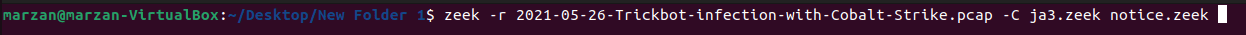
\includegraphics[width=1\linewidth]{images//ja3image/21.PNG}
    \caption{run pcap file with ja3.zeek and notice.zeek script}
    \label{fig:enter-label}
\end{figure}

\begin{itemize}
    \item The ssl.log file is examined to review detailed TLS handshake records and associated JA3 hashes generated during the simulation.
\end{itemize}
\begin{figure}[H]
    \centering
    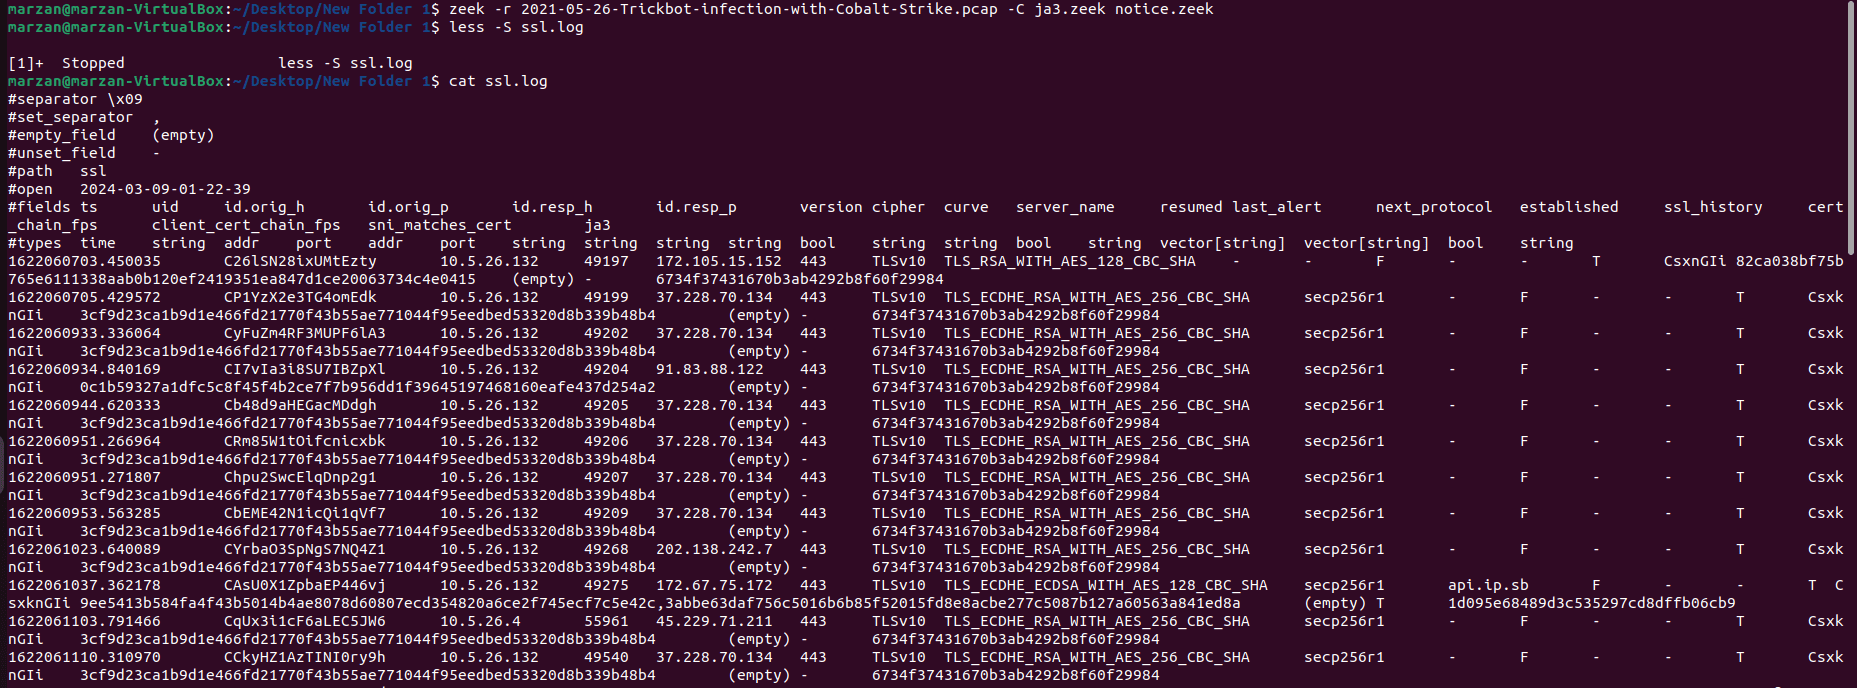
\includegraphics[width=1\linewidth]{images//ja3image/22.PNG}
    \caption{ssl.log}
    \label{fig:enter-label}
\end{figure}

\begin{itemize}
    \item Specific JA3 hash fields are extracted from the ssl.log for focused analysis.
\end{itemize}
\begin{figure}[H]
    \centering
    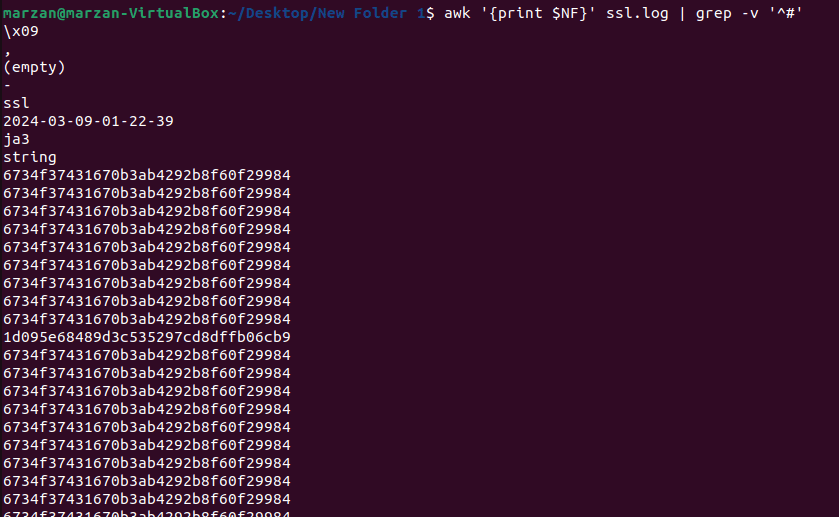
\includegraphics[width=1\linewidth]{images//ja3image/25.PNG}
    \caption{ja3 entries}
    \label{fig:enter-label}
\end{figure}

\begin{itemize}
    \item The ssl.log entries are visualized in BRIM, offering a tabular representation of SSL transactions and JA3 hashes
\end{itemize}
\begin{figure}[H]
    \centering
    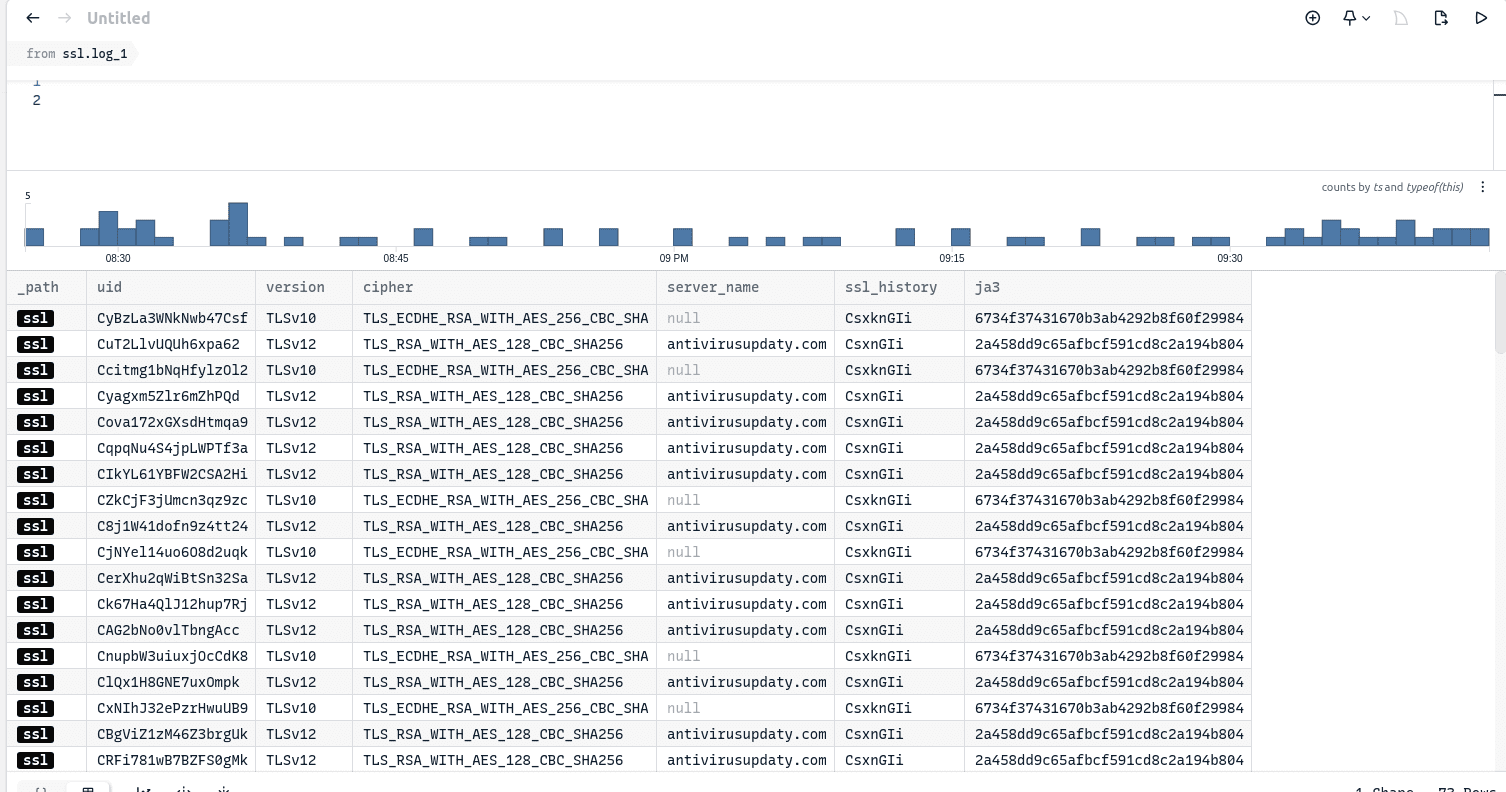
\includegraphics[width=1\linewidth]{images//ja3image/31.PNG}
    \caption{ssl.log in BRIM}
    \label{fig:enter-label}
\end{figure}

\begin{itemize}
    \item  The notice.log file is checked for Trickbot hash detection alerts, confirming the identification of malicious communications.\\\\
    JA3 = 6734f37431670b3ab4292b8f60f29984 ( Fingerprint of Trickbot )
\end{itemize}
\begin{figure}[H]
    \centering
    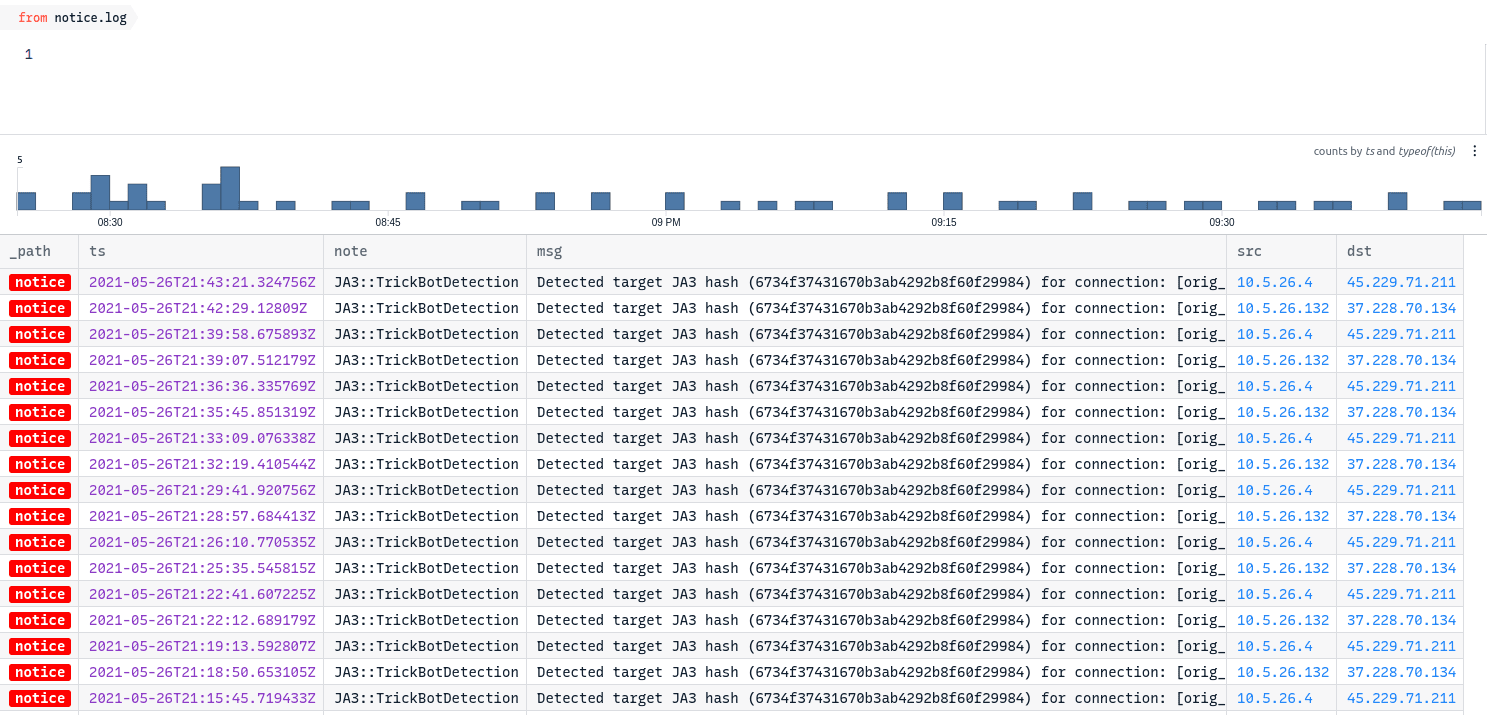
\includegraphics[width=1\linewidth]{images//ja3image/32.PNG}
    \caption{notice.log in BRIM}
    \label{fig:enter-label}
\end{figure}
